\section{Proposed Method}\label{sec:method}

%Now comes the ``beef'' of the paper, where you explain what you
%did. Again, organize it in paragraphs with titles. As in every section
%you start with a very brief overview of the section.

%For this class, explain all the optimizations you performed. This mean, you first very briefly
%explain the baseline implementation, then go through locality and other optimizations, and finally SSE (every project will be slightly different of course). Show or mention relevant analysis or assumptions. A few examples: 1) Profiling may lead you to optimize one part first; 2) bandwidth plus data transfer analysis may show that it is memory bound; 3) it may be too hard to implement the algorithm in full generality: make assumptions and state them (e.g., we assume $n$ is divisible by 4; or, we consider only one type of input image); 4) explain how certain data accesses have poor locality. Generally, any type of analysis adds value to your work.

As a baseline we used the libDAI library \cite{Mooij_libDAI_10} which provides an implementation for loopy belief propagation using the max residual updating scheme. With the library, it was simple to implement the recommendation system as proposed in \cite{Ha:2012:TRT:2396761.2398636}.

\mypar{Code structure}
Figure \ref{overviewflow} shows a high-level overview of the code structure. After an initialization phase the BP algorithm is invoked which loops until a specified maximum number of iterations is reached, the maximum residual becomes zero or the change in the updated messages is smaller than some specified tolerance. In every iteration, findMaxResidual is called to determine the message that should be updated next (by updateMessage). The actual update step goes quickly, because it only assigns newMessage to message. The costly part of the algorithm is the re-computation of newMessage for all neighbouring nodes that are affected by the change. To do so, calcNewMessage is called for every candidate, which first computes a product over all incoming messages (calcIncomingMessageProduct) and then marginalizes this product of messages over all other variables (marginalizeProductOntoMessage). Note that the residual is simply $||\mathtt{message}-\mathtt{newMessage}||_\infty$. 

%\lstset{basicstyle=\tiny\ttfamily}
%\begin{table}
%\begin{lstlisting}
%init()
%while (not done)
%   messageToUpdate <-- findMaxResidual;
%\end{lstlisting}
%\caption{Pseudo code for Residual BP}
%\end{table}

The methods that get called the most often are updateResidual, calcIncomingMessageProduct and marginalizeProductMessage. Hence, our optimizations will mostly focus on these.

\begin{figure}\centering
    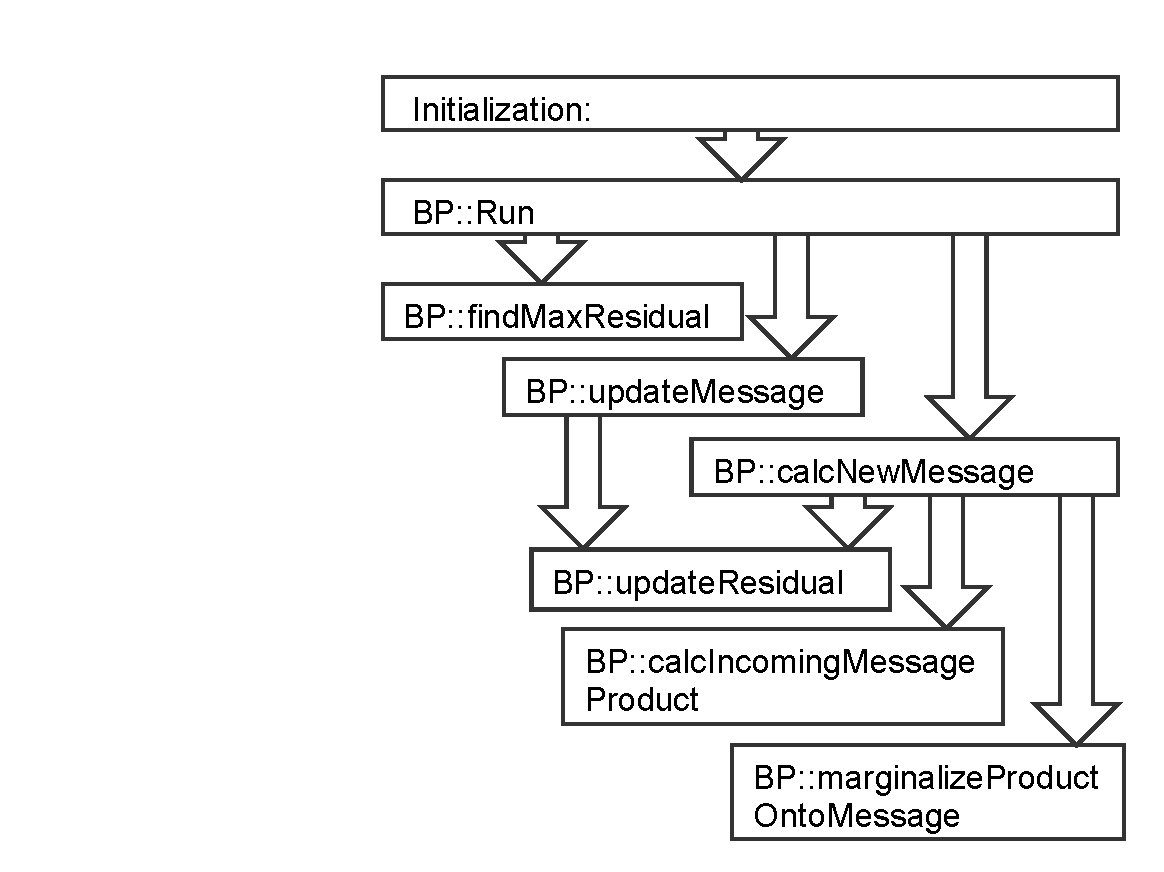
\includegraphics[scale=0.5, trim={6.45cm 0cm 0 1.25cm},clip]{graphics/loopybp-compact.pdf}
  \caption{Flow (top to bottom) of our program. Arrows denote that a methods gets called from an other, BP is the namespace used for all functions that deal with belief propagation.\label{overviewflow}}
\end{figure}


\mypar{Optimizations}
The optimization of the code was performed iteratively, driven by insights from analyzing and profiling the code. In a first phase, we focused on general optimizations that would not change the interfaces and generality of the implementation. In a second phase the special property of the recommender system were exploited, trading in generality for speed and interfering drastically with the interface of the library.

(TODO: rewrite) 
In both phases, we started off by reducing the Op counts, without considering the computational intensity. We then profiled our code to find critical points where we could optimize memory access patterns or reorder operations to increase the computational intensity. This was also the point where we decided to switch from double to single precision which decreased our accuracy slightly but gave us an significant boost for the runtime. %TODO: How much?
As a final step we considered vectorization which gave us only a very small speed-up. We will now explain all our optimizations in more detail.

We would also like to point out that we had to decide whether we wanted to work in a logarithmic domain. This would have enabled us to express the product over the messages as a sum, often making it less likely to suffer from numerical rounding errors and sometimes making the computation faster. We tested this option but found that in our case the accuracy did not improve. Furthermore the runtime increased slightly because we had to deal with the additional overhead of transforming the values to/from the log domain. We, therefore, decided to not utilize this option.

\mypar{Phase 1: General optimizations}
% -- Optimize calculation of product -- 
The first observation was that the incoming message product is recomputed each time a message (single factor in the product) gets updated. This is expensive because the product often goes over a hundred factors. To avoid the re-computation we computed the product once over all messages. Whenever a message changed we then updated the product by multiplying it with the new message and dividing it by the old message. This gave us an speed-up of 1.6 reducing the runtime of the algorithm from 80 to 50 seconds for our big dataset.

%TODO: sicherstellen, ziemlich früh zu erwähnen, dass alle performance angaben stark vom datensatz (size AND shape) abhängen. Konvention: wir beziehen den speedup immer auf den datensatz u1, den wir zu beginn immer verwendet haben

% -- C++ refactoring --
The baseline libDAI favours readability over performance. Encouraged by evidence from the profiler, a subsequent optimization step consisted in the re-factoring of the code base with the main objective to reduce memory ops. The biggest improvement we achieved was modifying functions to operate in-place. Another improvement consisted in the creation of buffers for intermediate results and to avoid superfluous creation and destruction of data. 
By applying memory-friendly C++ we achieved an overall speed-up of about a factor 2.0 (reference data set u1).

%-- Switch to single precision
At this stage, the code was memory bound. To further reduce memory traffic, we enabled the support for single floating point precision. However, because the sum-product algorithm requires to calculate products with a large number of factors (the actual number is defined by the degree of the nodes in the factor graph), a trade-off approach was chosen: the calculation of products was still performed with double precision, but the messages could be stored in single precision because they are always normalized. Nevertheless this reduced our precision which also meant that we had to adjust the convergence tolerance. This had a big impact on the number of message that needed to be send. For our reference dataset the number of messages was reduced by a factor of 6. But the total speed-up was around 12, this means a net speed-up of 2 was achieved, which in this case is equivalent to an equally increase of the operational intensity. Our code can still be compiled for both single and double precision (storage) through a compiler flag.

\mypar{Phase 2: Specific optimizations}
%-- More efficient storage of messages.
For every iteration, a possibly large number of messages is read and stored. Therefore, it is beneficial to reduce the number of message lookups. Because a message $m$ represents a normalized probability distribution that satisfies $\sum_i=1^N m_i = 1$, it suffices to store only $N-1$ values for every message. Taking into account that the recommender system uses variables with only two states (like/dis-like), the amount of bytes required to store a message can be divided by a factor of two. 

%-- Exploit the special pattern how messages are updated
An analysis of the pattern how message products are calculated revealed a calculation pattern that is specific for the factor graph of the recommender system. Hardcoding this pattern is beneficial because one can save an index lookup that is required for the generic case. To be more specific: calcIncomingMessageProduct\_0101\_0011 calculates the optimized (unmarginalized) product coming from factor I required to update variable i. 
Technically, the optimization is comparable with a loop unrolling where the innermost loop necessary for the index lookup is flattened away.

The two specific optimization steps improved runtime by a factor of two (reference data set u1).

%-- Precalculate reciprocals
The first optimization (pre-calculation of message products, with later division of a message) increased the pressure on the floating point division unit. As our investigations pointed out, this issue turned into one of the major bottlenecks of our code. By pre-calculating reciprocals (“1/message”) the dependency on the fp division unit could be reduced slightly.  

%-- Vectorization
To further reduce the dependency on the division unit, we decided to introduce vectorization.
Unfortunately, the fast but less accurate \_mm\_rcp\_ps is not applicable for our use case because of precision problems, so the precalculation is performed with ordinary division.


%As important as the final results is to show that you took a structured, organized approach to the optimization and that you explain why you did what you did.

%Mention and cite any external resources including library or other code.

%Good visuals or even brief code snippets to illustrate what you did are good. Pasting large amounts of code to fill the space is not good.
